\chapter{Implementation}
\label{sec:implementation}

\section{Frontend}
\subsection{Architecture}

\begin{figure}[H]
\centering
\caption{Frontend codebase structure}
\label{fig:frontend_structure}
\resizebox{0.55\textwidth}{!}{%
\begin{forest}
  for tree={
    font=\ttfamily\small,
    grow'=0,
    child anchor=west,
    parent anchor=south,
    anchor=west,
    calign=first,
    inner xsep=4pt,
    edge path={
      \noexpand\path [draw, \forestoption{edge}]
        (!u.south west) +(7.5pt,0) |- (.child anchor)\forestoption{edge label};
    },
    before typesetting nodes={
      if n=1{insert before={[,phantom]}}{},
    },
    fit=band,
    before computing xy={l=15pt},
  }
  [frontend/
    [api/
      [base.js]
      [documents.api.js]
      [models.api.js]
      [projects.api.js]
      [document-model-links.api.js]
      [...api.js]
    ]
    [modules/
      [document/
        [file.js]
        [selection.js]
      ]
      [model/
        [wfadaptor.js]
        [endpoints/]
        [themes/]
        [utils/]
      ]
    ]
    [pages/
      [home/
        [init.js]
        [ui/
          [projects.ui.js]
          [project-creation.ui.js]
          [dashboard.ui.js]
        ]
      ]
      [stats/
        [init.js]
        [store.js]
        [ui/]
      ]
      [workspace/
        [init.js]
        [services/
          [workspace.service.js]
          [document.service.js]
          [model.service.js]
        ]
        [store/
          [workspace.store.js]
          [documents.store.js]
          [document-viewer.store.js]
          [models.store.js]
          [model-editor.store.js]
          [project-graph.store.js]
        ]
        [ui/]
        [utils/]
        [css/]
      ]
    ]
    [shared/
      [utils/
        [{url.js, dom.js, date.js}]
        [{store.js, ui.js, number.js}]
      ]
      [widgets/
        [inline-editor.js]
        [...js]
      ]
    ]
    [{index.html, workspace.html}]
    [{....html}]
    [constants.js]
  ]
\end{forest}%
}
\end{figure}

The frontend was implemented as a native web application using JavaScript, HTML, and CSS. This decision follows the design constraint defined in the previous chapter and keeps the client architecture lightweight while still allowing fine-grained control over document rendering and model-editor integration. In implementation terms, the codebase is organized into several layers. The HTML entry pages, such as \texttt{index.html} and \texttt{workspace.html}, provide page-specific containers. Each page then loads an initialization module that validates URL state, imports the required UI modules, and starts the runtime flow. The main workspace entry point is responsible for validating the project identifier, loading the page-specific UI modules, and triggering the initial data load for the current project.

The structure shown in Figure~\ref{fig:frontend_structure} reflects the realized separation of concerns. The \texttt{api} folder encapsulates communication with the backend REST endpoints. The \texttt{pages} folder contains the page-level composition logic, especially the workspace page where the end-to-end modelling workflow takes place. Inside the workspace page, the implementation is divided into services, stores, UI modules, utilities, and CSS resources. The \texttt{modules} folder contains domain-specific logic for document handling and process-model rendering, while \texttt{shared} provides reusable utilities such as generic state management, DOM helpers, and small widgets. This organization proved sufficient without introducing a frontend framework, because the application logic is centered on a small number of coordinated views rather than on a very large component tree.

At runtime, the workspace page acts as the central frontend container. After the project is validated, the workspace service loads the metadata for documents, models, and subprocess relationships, initializes the corresponding stores, and selects an initial document if available. Subsequent user actions, such as opening a document version, generating a model, switching to a historical version, or navigating to a subprocess, are then handled through the same orchestration layer. As a result, the frontend behaves as a workspace-centered reactive system rather than as a collection of isolated pages.

The simplified runtime flow is shown in Figure~\ref{fig:imp_frontend_workspace_flow}. It illustrates how page initialization, service orchestration, and store updates are chained during startup.

\begin{figure}[H]
  \centering
  \caption{Simplified workspace initialization flow}
  \label{fig:imp_frontend_workspace_flow}
  \begin{lstlisting}[language=Python]
projectId = readProjectIdFromUrl()
if not projectId:
    redirectToHome()

validateProject(projectId)
loadWorkspaceUiModules()

documentsMeta, modelsMeta, subprocessLinks = fetchProjectComponents(projectId)
documentsStore.init(documentsMeta)
modelsStore.init(modelsMeta)
projectGraphStore.init(documentsMeta, modelsMeta, subprocessLinks)

if documentsMeta is not empty:
    latestDocument = documentsMeta[-1]
    documentService.loadVersion(latestDocument.latestVersionId)
    workspaceStore.setViewedDocument(latestDocument)
  \end{lstlisting}
\end{figure}

\subsection{State Management}
To coordinate the document list, document viewer, model editor, and project graph without introducing strong coupling between them, the frontend implements a lightweight publish-subscribe state-management mechanism. The base implementation is intentionally small and is shown in Figure~\ref{fig:imp_frontend_pubsub_store}. Each store keeps its internal state and a set of subscriber callbacks. Whenever the state changes, a patch object is emitted to all subscribers. This design keeps updates explicit and avoids hidden side effects in the UI layer.

The store abstraction is specialized for the needs of the workspace. A generic entity store manages collections by identifier and supports operations such as add, update, delete, selection, and bulk-edit state. On top of it, a version-aware entity store adds support for version histories and latest-version resolution, which is required by both documents and process models. Concrete stores then hold the active workspace context, document metadata, rendered document content, model metadata, model-editor state, and the project graph. In practice, this means that UI modules can subscribe only to the changes relevant to them, while services remain responsible for orchestrating state transitions across multiple stores.

This custom pub-sub approach was chosen because the frontend requires reactive synchronization across multiple panes, but does not require the full abstraction overhead of a large framework. It also maps well to the workspace workflow. For example, switching the displayed document updates the viewed-document state, clears obsolete viewer state, loads the content and links of the selected version, and can optionally reset the model editor if the context has changed. The patch-based notification model makes these transitions observable and keeps the data flow understandable during development and debugging.

\begin{figure}[H]
  \centering
  \caption{store implementation}
  \label{fig:imp_frontend_pubsub_store}
  \begin{lstlisting}[language=JavaScript]
export class Store {
  constructor(initialState = {}) {
    this.state = { ...initialState };
    this.subscribers = new Set();
  }

  subscribe(fn) {
    this.subscribers.add(fn);
    return () => this.subscribers.delete(fn);
  }

  notify(patch) {
    this.subscribers.forEach((fn) => fn(patch));
  }
}
  \end{lstlisting}
\end{figure}

\subsection{Document Processing}
Document upload is handled partly on the frontend so that heterogeneous source formats can be normalized before they enter the main interaction flow. The implementation accepts PDF, DOC, DOCX, and plain-text input. For Word documents, the content is converted to HTML and inserted into the viewer as structured markup. For PDF files, the preprocessing logic is more involved because the browser cannot directly provide a robust text structure for later selection and re-anchoring.

The PDF pipeline first extracts positioned text items from each page and normalizes their geometry, font size, and textual content. These low-level items are then grouped into lines according to their vertical alignment, after which several heuristics classify the resulting lines as headings, list items, or normal paragraph text. Adjacent lines are further merged into blocks based on indentation, vertical spacing, and font changes. Finally, the processed blocks are rendered as semantic HTML sections. This transformation is necessary because later frontend operations depend on stable DOM text ranges. Selection serialization, overlay rendering, and re-anchoring all become significantly more reliable when the input is available as normalized HTML instead of raw file data.

This preprocessing step is also an implementation trade-off. Some document layout information is simplified during conversion, especially in PDF files with complex formatting. However, for the purpose of document-based process modelling, preserving a readable and structurally coherent text flow is more important than preserving exact visual fidelity. The generated HTML therefore acts as an interaction-oriented representation of the document rather than as a pixel-accurate viewer.

\subsection{Text Selection Rendering}
One of the central frontend mechanisms is the transformation of browser text selections into persistent, version-aware linkable objects. When the user selects a passage in the document viewer, the range is serialized into a text-position selector together with a text-quote selector. This combination follows the idea of robust text anchoring from the W3C Web Annotation Model \cite{w3c_annotation_model}. The text-position selector provides an exact range within the current text stream, while the text quote preserves the selected wording and can later support validation or re-anchoring after document updates.

Figure~\ref{fig:imp_frontend_selection_serialization} shows the core implementation used to convert a browser range into a persistent selector object. This code is small, but it is central because it defines the representation that later connects document passages, stored links, and model generation requests.

\begin{figure}[H]
  \centering
  \caption{Core implementation of selection serialization}
  \label{fig:imp_frontend_selection_serialization}
  \begin{lstlisting}[language=JavaScript]
export function serializeRange(range) {
  const root = getRoot();
  const textPosition = textPos.fromRange(root, range);
  const textQuoteSelector = textQuote.fromTextPosition(root, textPosition);

  return {
    textPosition,
    textQuote: textQuoteSelector,
  };
}
  \end{lstlisting}
\end{figure}

When a stored selection has to be displayed again, the frontend resolves the serialized selector back into a DOM range. This deserialization step is essential for loading existing links, reviewing older model versions, and visualizing the relation between documents and process models. The serialized form therefore acts as the boundary between the persistent representation stored by the system and the transient range object used by the browser at runtime.

\subsubsection{Virtual Overlay Strategy}
The visual rendering of selections is implemented as a virtual overlay rather than by directly wrapping the underlying text nodes. The selection module first collects client rectangles for the text range, filters out non-renderable rectangles, de-duplicates geometrically equivalent rectangles, and removes container rectangles that would otherwise lead to oversized highlight areas. An additional refinement is applied when a browser returns a single suspiciously tall rectangle for a multi-line selection. In this case, the implementation tokenizes the text and reconstructs more precise line-level rectangles. The resulting geometry is then used to draw separate overlay elements above the document content.

This strategy was chosen for two reasons. First, directly mutating the source DOM would complicate later re-rendering, selection updates, and version switches. Second, the document content is imported from heterogeneous sources, so keeping the original HTML structure untouched reduces rendering side effects. The overlay-based approach therefore decouples interaction feedback from the content representation while still allowing precise highlighting.

\subsubsection{Link Update Detection}
The frontend also distinguishes between semantic changes in a linked selection and purely visual updates. When a link draft is compared against the current rendered selections, the implementation separately evaluates the text-position and text-quote information on the one hand and presentation properties such as highlight color or review status on the other hand. This leads to three explicit states: no change, color-only change, and text-changed. The distinction is important for document-version updates because a purely visual modification should not invalidate the semantic relation between a document passage and a model, whereas a changed text anchor may require review or re-anchoring.

\subsection{Modeling}
The modeling flow is implemented as a coordinated interaction between the document viewer, the model service, and the model editor state. Once the user has selected one or more passages, the selected text is aggregated and optionally combined with an additional prompt. This generation input is then passed to the model service, which manages the asynchronous request to the LLM-backed generation endpoint, updates the editor status messages, and stores generation progress in the editor state.

The result of this process is model data represented as XML in the format required by the integrated CPEE-based editor. The frontend loads this data into the model editor store and renders it in the editing pane. At the same time, the service layer keeps the relation to the originating document version available so that the currently edited model can be synchronized with the document context. This is especially important when the user switches between new models, existing models, regenerated models, and historical versions.

Model versioning is therefore handled directly in the frontend interaction logic. A model may be newly generated from a fresh selection, regenerated from the linked document passage, or refined using an additional prompt. In all cases, the service layer maintains the distinction between the latest editable version and historical versions used for review. This version-aware coordination is one of the reasons why the modeling logic is implemented in a dedicated service rather than directly inside the UI modules.

\subsection{Rendering Customization}
Instead of implementing a process-model editor from scratch, the frontend reuses the CPEE layout and rendering infrastructure and extends it where necessary. The most important adaptation is the customization of the workflow adaptor base used by the renderer. The customized layer intercepts interactions with call nodes and subprocess nodes and dispatches additional browser events such as call-clicked, subprocess-hovered, subprocess-unhovered, and subprocess-double-clicked.

These custom events provide the bridge between the generic renderer and the specific needs of the document-based modeling workspace. In the implemented system, subprocesses are not only visual model elements but also navigable links to other models within the same project. The frontend therefore needs richer interaction signals than those originally provided by the renderer alone. By adding this customization layer, the system can support workspace-specific behavior, such as subprocess navigation and context-sensitive highlighting, while still preserving the original rendering engine and its XML-based editing capabilities.

Taken together, the frontend implementation is centered on keeping multiple representations synchronized: imported document content, persistent anchored selections, model versions, and interactive process visualizations. The layered organization, lightweight pub-sub stores, document normalization pipeline, overlay-based selection rendering, and renderer customization jointly enable the end-to-end workspace workflow described in the solution design.
\section{Backend}
\subsection{Architecture}
The backend was implemented with Node.js and Fastify. This choice matches the lightweight architecture of the frontend while providing a practical HTTP server, straightforward route registration, and built-in support for request and response schema validation. At application startup, the server creates the required persistence directories, registers CORS and static-file handling, and mounts the domain-specific route modules for projects, documents, models, and document-model links. In this sense, the backend acts both as an API server and as the delivery layer for the frontend and persisted document/model assets.

The realized backend structure follows a layered route-service-repository pattern. Route modules define the REST endpoints and bind them to JSON schemas. Service modules contain the business logic, such as creating new document versions, copying or updating document-model links, generating model-version metadata, recording generation attempts, and handling soft-delete or restore operations. Repository modules encapsulate persistence details and isolate SQL access from the service layer. This separation keeps the HTTP layer small and allows the more involved versioning and synchronization logic to be implemented in a reusable way.

The schema layer is particularly important because the system processes structured selection data exchanged with the frontend. As shown in Figure~\ref{fig:imp_backend_schema_example}, selectors are validated explicitly before entering the service logic. This reduces the risk of malformed anchoring data and keeps the contract between frontend and backend stable. The same pattern is applied across modules for documents, models, and links, where both request bodies and route parameters are validated before processing.

\begin{figure}[H]
  \centering
  \caption{Example JSON schema used in the backend for text quotes}
  \label{fig:imp_backend_schema_example}
  \begin{lstlisting}[language=JavaScript]
const textQuoteSchema = {
  type: "object",
  required: ["exact"],
  additionalProperties: false,
  properties: {
    exact: { type: "string" },
    prefix: { type: "string" },
    suffix: { type: "string" },
  },
};
  \end{lstlisting}
\end{figure}

The backend implementation combines relational persistence with file-based storage. Metadata such as projects, documents, models, versions, links, subprocess references, generation attempts, and version events are stored in SQLite via the \texttt{better-sqlite3} library. By contrast, large document contents and model XML payloads are stored as files in the persistence directory. This hybrid design is deliberate. Relational storage supports queries over versions, links, and project-level statistics, whereas file storage avoids placing large HTML and XML payloads directly into the relational schema. A shared base repository class provides reusable create, read, and update operations, including camelCase to snake\_case mapping and JSON serialization for structured columns.

The service layer implements the application-specific behavior that the frontend depends on. For example, when a new document version is created, the backend stores the new content, updates the latest-version pointer, copies the latest link information to the new document version, and schedules the corresponding model-link synchronization work. Likewise, when a new model or model version is created, the backend persists the XML payload, updates latest-version references, injects DBPM-specific metadata into the model data, stores the related document-model link, and records monitoring information such as generation attempts or manual update events. These operations involve several repositories at once, which is why they are implemented at the service level rather than in individual route handlers.

The backend also implements several cross-cutting concerns required by the overall system design. Soft deletion is used for projects, documents, subprocess links, and models so that historical information can remain available for restoration and analysis. Logging is handled as a dedicated module and is invoked from the service layer when relevant lifecycle actions occur. The project service additionally exposes aggregated component endpoints that bundle document metadata, model metadata, and subprocess links into a single response tailored to the workspace frontend. The resulting architecture is shown in Figure~\ref{fig:imp_backend_com}. Rather than exposing the database directly to the client, the backend serves as the consistency layer that preserves version relations, link integrity, and monitoring data across the full modelling workflow.

\begin{figure}[H]
    \centering
    \caption{Backend Component} 
    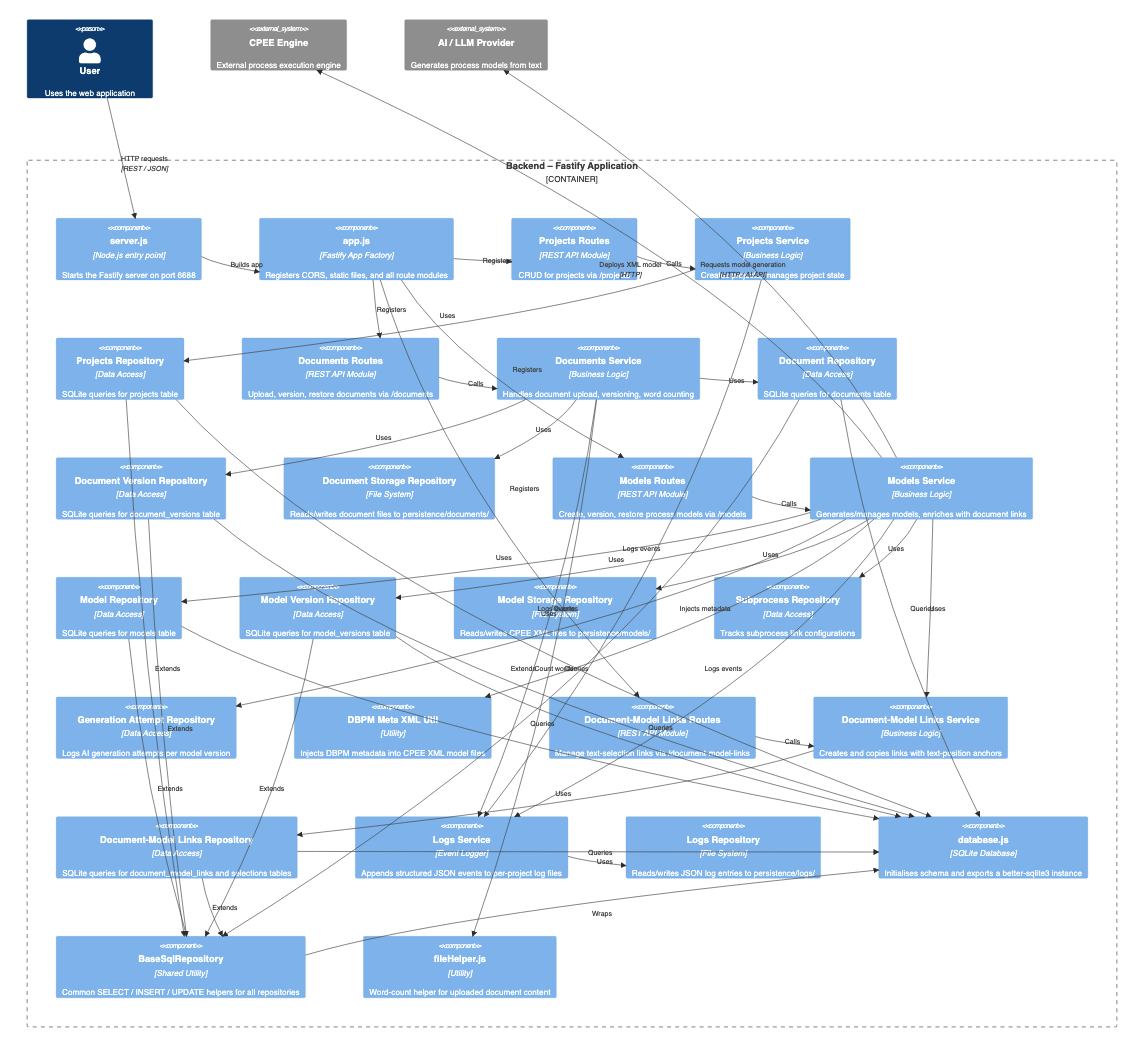
\includegraphics[width=0.8\textwidth]{images/imp_backend_com.png}
    \floatfoot{The backend component of the document-based process modeling tool.}
    \label{fig:imp_backend_com}
\end{figure}
\section{Database Schema}

Firstly, Project, Document, Model and Document Model Link are the minimal tables needed to support the proposed system. It is also how the system was implemented when it first adopted the database. The Document and Model tables were used to store metadata like name, words count of a document. Theoretically, the Document Model Link table can be stored as an attribute within the model version, since the system is currently designed to allow one model to be derived from only one document. But it is a decision made very early to store it in a separate table to easily support a potentially many-to-many (M2M) relationship in the future.

The Model Version table is added when the model versioning feature is about to be implemented. The Document Version table is added at the same time to prepare for supporting the Document Update feature, as both tables follow a similar logic at the DB operation level. 

The Subprocess Link table is an additional table used to support the Project Graph. As this relationship information has been embedded in Model Data, the model visualization itself does not need this data. However, for the project graph, the relationship is hard to be parsed from the model data; therefore, such a table is designed to easily retrieve the process-subprocess relationship.

The Selection and Selection History tables are then added when designing the Document Update feature. Before the selection data (e.g., color, position) for a Document Model Link is stored as an attribute in the format of a stringified JSON object. To better support auto-reanchoring for document upload, Selection and Selection History are designed as separate tables. The separate Selection table can make selection data easier to retrieve for reanchor operations. Besides, a Selection History is designed to make it easier to track the quality of reanchor. 

Finally, the Generation Attempt and Version Event tables are the two tables designed to monitor the system behavior. The Generation Attempt table is used to monitor the accept/decline decision for the LLM-generated output. The Version Event is mainly to store the manual edit behavior or a system auto-update behavior, e.g., selection reanchor for document update. 